\section{Introduction}

The purpose of these notes is to provide a short introduction to \textbf{Approximate Message Passing (AMP) algorithms} and \textbf{replicas} computation, that we illustrate for \textbf{committee machines}, that are a simple generalization of \textbf{generalized linear models}. For more details, see in particular the references \cite{mezard1987spin, Castellani2005, Barbier2017b, Yedidia2001, Krzakala2012, Zdeborova2016, Lesieur2017}.


\subsection{Model}

We revisit the so-called \emph{teacher-student} scenario from statistical physics \cite{Patarnello_1987,gardner1989three,tishby89,Sompolinsky1990,seung1992statistical,watkin1993statistical,Gyorgyi2001}. 
We assume that the synthetic dataset is generated by a \emph{teacher} model. 

\subsubsection{Data}

We assume that the matrix of data inputs $\mat{X} \in \bbR^{\nsamples \times \ndim }$, that contains $\nsamples$ $\ndim$-dimensional samples, is drawn \aclink{i.i.d} with distribution $\rP_\x(\mat{X}) = \displaystyle \prod_{i,\mu=1}^{\ndim, \nsamples} \rP_\x(x_{\mu i})$.\\
For simplicity, we will consider them to be \aclink{i.i.d} Gaussian with zero mean and unit variance: $\forall \mu \in \lb \nsamples \rb, \vec{x}_{\mu} \sim \mN_{\vec{x}}\(\vec{0}, \mat{I}_{\ndim}\)$.

\subsubsection{Teacher - Planted solution}
Moreover, we draw a \textbf{planted solution} $\mat{W}^\star$ from a separable distribution (across the input dimension) $\rP_{\w^\star}(\mat{W}^\star) = \prod_{i=1}^\ndim \rP_{\w^\star}\(\vec{w}_i^\star\)$. Therefore the weights could possibly be correlated across the second dimension.


\begin{figure}[htb!]
\centering
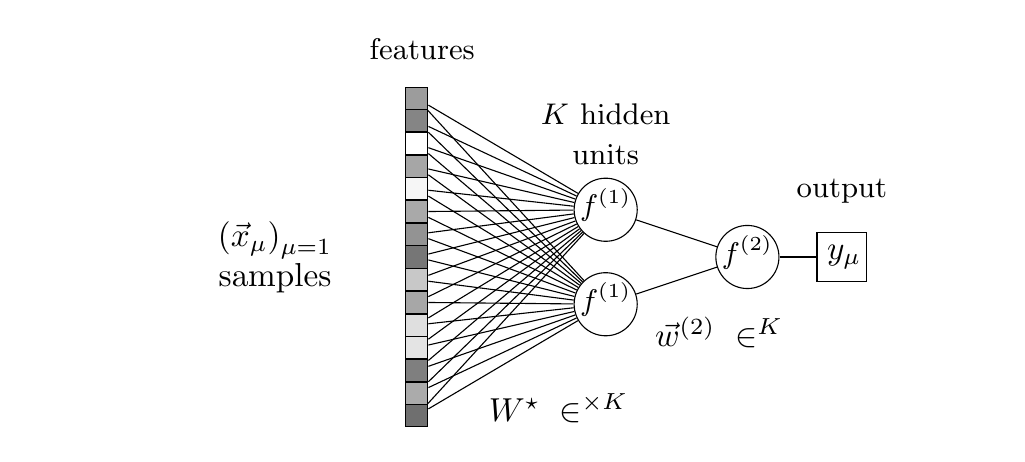
\begin{tikzpicture}[scale=1.2, every node/.style={transform shape}]
    \tikzstyle{factor}=[rectangle,minimum size=4pt,draw=black, fill opacity=1.]
    \tikzstyle{latent}=[circle,minimum size=19pt,draw=black, fill opacity=1.,fill=white]
    \tikzstyle{output}=[circle,minimum size=19pt,draw=black, fill opacity=1.,fill=white]
        \tikzstyle{noise}=[circle,minimum size=18pt,draw=black, fill opacity=1.,fill=white]
    \tikzstyle{output_y}=[rectangle,minimum size=15pt,draw=black, fill opacity=1.,fill=white]
    \tikzstyle{annot} = [text width=3cm, text centered]
    \tikzstyle{annot} = [text width=3cm, text centered]
    \tikzstyle{annotLarge} = [text width=5cm, text centered]
    \def\NX{15}
    \def\NK{2}
    \def\NY{1}
    \def\middle{0}
    \foreach \i in {1,...,\NX}
     	  \pgfmathparse{0.9*rnd+0.3}
          \definecolor{MyColor}{rgb}{\pgfmathresult,\pgfmathresult,\pgfmathresult}
    	\node[factor, fill=MyColor] (X-\i) at (\middle 0, 0.24*0.5*\NX+0.12 - 0.24*\i ) {}; 
    \foreach \k in {1,...,\NK}
    	\node[latent] (K-\k) at (2,\middle  \k - 1.5) {}; 
    \foreach \y in {1,...,\NY}
    	\node[output] (Y-\y) at (3.5,0) {}; 	
    \node[output_y] (Y-2) at (4.5,0) {}; 
    
    \foreach \i in {1,...,\NX}
    	\foreach \k in {1,...,\NK}
    		\path[-] (X-\i) edge (K-\k);
   	\foreach \k in {1,...,\NK}
    	\foreach \y in {1,...,\NY}
    		\path[-] (K-\k) edge (Y-\y);
    \path[-] (Y-1) edge (Y-2);
    \node[annotLarge] at (-1.5,0) {$(\vec{x}_{\mu})_{\mu=1}^{\nsamples}$ \\ samples};
    \node[annot] at (1.5,-1.6) {$\mat{W}^\star \in \bbR^{\ndim \times K}$}  ;
    \node[annot] at (4.525,0) {${y_{\mu}}$}  ;
    \node[annot] at (3.2,-0.8) {$\vec{w}^{(2)}\in\bbR^{K}$}  ;
    \node[annot] at (2,-0.45) {\small $ f^{(1)}$}  ;
    \node[annot] at (2,0.55) {\small $ f^{(1)}$}  ;
    \node[annot] at (3.5,0.05) {\small $ f^{(2)}$}  ;
    \node[annot] at (0,2.2) {\small $\ndim$ features}  ;
    \node[annot] at (2,1.3) {\small $K$ hidden\\ units}  ;
    \node[annot] at (4.5,0.7) {\small output}  ;
	\end{tikzpicture}	
	\caption{Illustration of the \emph{committee machine}: it is one of the simplest models belonging to the considered model class \eqref{model}, and on which we focus to illustrate our results. It is a two-layers neural network with sign activation functions $f^{(1)},f^{(2)}=\sign$ and weights $\vec{w}^{(2)}$ fixed to unity. It is represented for $K=2$.}
	\label{fig:committee}
\end{figure}


\subsubsection{Channel}

The labels are then generated by multiplying the data matrix $\mat{X}$ and the planted weights $\mat{W}^\star$ and passing their product to a \textbf{channel} $\varphi_\out$, acting component-wise, according to:

\begin{equation}
\label{model}
\vec{y} = \varphi_\out \( \left\{ \frac{1}{\sqrt{\ndim}} \mat{X} \vec{w}_k^\star \right \}_{k=1}^K \) ~~~\text{or}~~~ \vec{y} \sim \rP_\out \( \cdot \Big| \left\{ \frac{1}{\sqrt{\ndim}} \mat{X} \vec{w}_k^\star \right \}_{k=1}^K \)\, ,
\end{equation}
and illustrated in \Fig\ref{fig:committee} in the case of a committee machine with fixed weights $\vec{w}^{(2)}$ in the second layer.

The function $\varphi_\out : \bbR^{K} \mapsto \bbR$ represents a deterministic, or stochastic function associated to a probability distribution $\rP_\out$, applied component-wise to each sample. 

\begin{remark}
	Notice that the factor $\frac{1}{\sqrt{\ndim}}$ is present to insure that the variance of the input data is normalized to the unit.
\end{remark}


\subsubsection{Student}

The committee machine estimation problem consists of trying to fit the $\nsamples$ input-output observations $\{\mat{X}, \vec{y} \}\in \bbR^{\nsamples \times \ndim} \times \bbR^{\nsamples}$.\\

In the case the \textbf{student} has exactly the same architecture, namely $\mat{W}^\star \in \bbR^{\ndim \times K}$ and $\mat{W} \in \bbR^{\ndim \times K}$ have the same dimensionality and prior information $\rP_{\w^\star}=\rP_{\w}$, this setting is called the \textbf{Bayes-optimal setting}. Otherwise, it is called the \textbf{mismatched setting}.\\

In these notes, we focus on the \textbf{Bayes-optimal setting}, so that the committee machine estimation problem for the student committee machine (within the same hypothesis class and with weights $\mat{W}\in \bbR^{\ndim \times K}$) reduces to learn the teacher rule generated by the ground truth weights $\mat{W}^\star$ from the supervised dataset $\{\mat{X}, \vec{y} \}$.

\begin{remark}
	Committee machines are a simple vectorized generalization of \textbf{GLM}, whose estimation is performed simultaneously with $K \geq 1$.
\end{remark}


\subsection{Notations}
\begin{itemize}
	\item $\mat{X} \sim \rP_\x(\mat{X}) = \prod_{i=1, \mu=1}^{\ndim, \nsamples} \rP_\x(x_{\mu i})$
	\item $\vec{W} \in \bbR^{\ndim \times K}$ is the matrix of weights of the first layer with prior distribution: $\rP_\w(\mat{W}) = \displaystyle \prod_{i=1}^\ndim \rP_\w(\vec{w}_i)$
	\item $\vec{y} \in \bbR^{\nsamples}$ is a set of $\nsamples$ scalar observations generated according to \eqref{model}.
	\item Indices $\mu \in  \lb \nsamples \rb $ and $i \in \lb \ndim \rb$ correspond respectively to data samples and input dimensions.
	\item $\alpha \equiv \frac{\nsamples}{\ndim}$ with $\ndim, \nsamples \to \infty$ and in the limit where $\alpha= \Theta(1)$
	\item $\bxi$ will denote later a Gaussian vectorial variable such that $\bxi \sim \mN(\vec{0},\mat{I}_K)$
\end{itemize}

